\documentclass[a4paper,twocolumn,12pt]{article}
\usepackage[utf8]{inputenc}
\usepackage[MeX]{polski}
\usepackage{fullpage}
\usepackage[breaklinks=true]{hyperref}
\usepackage{amsthm}
\usepackage{ragged2e}
\usepackage{tikz}
\usetikzlibrary{calc,shapes,shapes.multipart,arrows,chains}
\usepackage{tikz-uml}

% ;;;;;;;;; colors ;;;;;;;;;;;;

\definecolor{Board}{RGB}{60,145,143}
\definecolor{DoubleWordBonus}{RGB}{239,174,154}
\definecolor{DoubleLetterBonus}{RGB}{141,201,240}
\definecolor{TripleLetterBonus}{RGB}{54,156,219}
\definecolor{Tile}{RGB}{247,225,190}
\definecolor{UniGreen}{RGB}{0,100,200}

% ;;;;;;;;; theorems ;;;;;;;;;;;;

\theoremstyle{definition}
\newtheorem{theorem}{Twierdzenie}
\newtheorem{definition}{Definicja}
\newtheorem{pro}{Dowód}

% ;;;;;;;;;;;;;;;;;;;;;;;;;;;;;;;;

\title{\LARGE{Zaawansowana sztuczna inteligencja do Scrabble} \\ \vspace{2mm} \large{Podstawy teoretyczne i~implementacja algorytmu}}
\author{Jakub Turek}
\date{\today}

\begin{document}

\maketitle

\begin{abstract}
Celem artykułu jest opisanie zbioru koncepcji, które posłużą do implementacji algorytmu sztucznej inteligencji grającego w~grę Scrabble w~języku polskim. Artykuł prezentuje zbiór teoretycznych informacji o~optymalnej strategii gry w~Scrabble. Ponadto zostały w~nim przedstawione elementy algorytmów zastosowanych w~aplikacjach Maven oraz Quackle. Autor wskazuje ich potencjalne słabe punkty i~sposoby usprawnienia, a~także prezentuje wyniki implementacji proponowanych poprawek.
\end{abstract}

\section*{Wstęp}

Scrabble to ,,gra słowna polegająca na układaniu na określonej planszy wyrazów z~losowanych liter''. \cite{scrabble_definition} Jest to bardzo ogólna definicja, którą należy uściślić. Scrabble jest grą przeznaczoną dla 2-4 osób. Akcesoriami do gry są: kwadratowa plansza o~stałym rozmiarze $15 \times 15$, torebka wypełniona płytkami, na których nadrukowane są litery oraz ich wartości punktowe, a~także stojaki, na których gracze umieszczają płytki, którymi w~danej chwili dysponują.

Gra rozgrywana jest w~turach. Zadaniem graczy jest układanie wyrazów na planszy w~taki sposób, aby tworzyły one poprawne słowa w~języku, w~którym prowadzona jest rozgrywka, w~układzie krzyżówkowym. Układ krzyżówkowy został przedstawiony na rysunkach \ref{fig:crossword_first} oraz \ref{fig:crossword_second}:

\begin{description}
 \item [Rysunek \ref{fig:crossword_first}] Pokazuje sytuację początkową obrazującą pewien moment rozgrywki.
 \item [Rysunek \ref{fig:crossword_second}] Pokazuje poprawny ruch zawodnika, który powoduje powstanie więcej niż jednego słowa. Wszystkie wyrazy utworzone przez jeden ruch muszą być poprawne. W~podanym przykładzie słowa ,,za'' i~,,masz'' są poprawne.
\end{description}

\begin{figure}[ht!]
	\begin{center}
			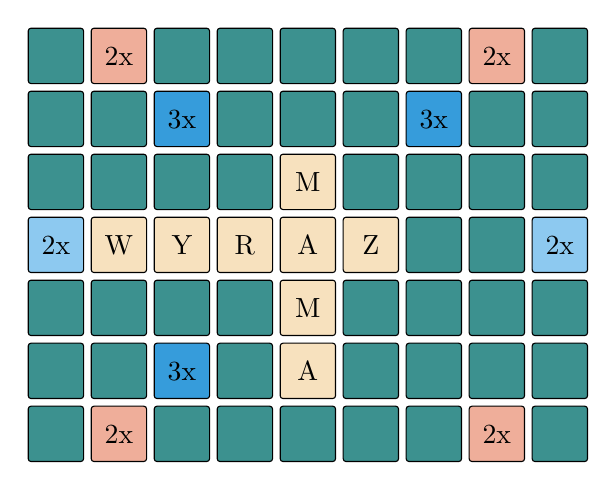
\begin{tikzpicture}
			\tikzstyle{every node}=[draw, shape=rectangle, rounded corners = 1pt, minimum width = 20pt, minimum height = 20pt, align=center, text height = 7pt];
			\node [fill=Board] at (-0.8, 0) {};
			\node [fill=DoubleWordBonus] at (0, 0) {2x};
			\node [fill=Board] at (0.8, 0) {};
			\node [fill=Board] at (1.6, 0) {};
			\node [fill=Board] at (2.4, 0) {};
			\node [fill=Board] at (3.2, 0) {};
			\node [fill=Board] at (4.0, 0) {};
			\node [fill=DoubleWordBonus] at (4.8, 0) {2x};
			\node [fill=Board] at (5.6, 0) {};
			\node [fill=Board] at (-.8, -.8) {};
			\node [fill=Board] at (0, -.8) {};
			\node [fill=TripleLetterBonus] at (0.8, -.8) {3x};
			\node [fill=Board] at (1.6, -.8) {};
			\node [fill=Board] at (2.4, -.8) {};
			\node [fill=Board] at (3.2, -.8) {};
			\node [fill=TripleLetterBonus] at (4.0, -.8) {3x};
			\node [fill=Board] at (4.8, -.8) {};
			\node [fill=Board] at (5.6, -.8) {};
			\node [fill=Board] at (-.8, -1.6) {};
			\node [fill=Board] at (0, -1.6) {};
			\node [fill=Board] at (0.8, -1.6) {};
			\node [fill=Board] at (1.6, -1.6) {};
			\node [fill=Tile] at (2.4, -1.6) {M};
			\node [fill=Board] at (3.2, -1.6) {};
			\node [fill=Board] at (4.0, -1.6) {};
			\node [fill=Board] at (4.8, -1.6) {};
			\node [fill=Board] at (5.6, -1.6) {};
			\node [fill=DoubleLetterBonus] at (-.8, -2.4) {2x};
			\node [fill=Tile] at (0, -2.4) {W};
			\node [fill=Tile] at (.8, -2.4) {Y};
			\node [fill=Tile] at (1.6, -2.4) {R};
			\node [fill=Tile] at (2.4, -2.4) {A};
			\node [fill=Tile] at (3.2, -2.4) {Z};
			\node [fill=Board] at (4.0, -2.4) {};
			\node [fill=Board] at (4.8, -2.4) {};
			\node [fill=DoubleLetterBonus] at (5.6, -2.4) {2x};
			\node [fill=Board] at (-.8, -3.2) {};
			\node [fill=Board] at (0, -3.2) {};
			\node [fill=Board] at (0.8, -3.2) {};
			\node [fill=Board] at (1.6, -3.2) {};
			\node [fill=Tile] at (2.4, -3.2) {M};
			\node [fill=Board] at (3.2, -3.2) {};
			\node [fill=Board] at (4.0, -3.2) {};
			\node [fill=Board] at (4.8, -3.2) {};
			\node [fill=Board] at (5.6, -3.2) {};
			\node [fill=Board] at (-.8, -4.0) {};
			\node [fill=Board] at (0, -4.0) {};
			\node [fill=TripleLetterBonus] at (0.8, -4.0) {3x};
			\node [fill=Board] at (1.6, -4.0) {};
			\node [fill=Tile] at (2.4, -4.0) {A};
			\node [fill=Board] at (3.2, -4.0) {};
			\node [fill=Board] at (4.0, -4.0) {};
			\node [fill=Board] at (4.8, -4.0) {};
			\node [fill=Board] at (5.6, -4.0) {};
			\node [fill=Board] at (-.8, -4.8) {};
			\node [fill=DoubleWordBonus] at (0, -4.8) {2x};
			\node [fill=Board] at (0.8, -4.8) {};
			\node [fill=Board] at (1.6, -4.8) {};
			\node [fill=Board] at (2.4, -4.8) {};
			\node [fill=Board] at (3.2, -4.8) {};
			\node [fill=Board] at (4.0, -4.8) {};
			\node [fill=DoubleWordBonus] at (4.8, -4.8) {2x};
			\node [fill=Board] at (5.6, -4.8) {};
		\end{tikzpicture}
		\caption{Fragment planszy. Gracze ułożyli kolejno słowa: ,,wyraz'' oraz ,,mama''.}
		\label{fig:crossword_first}
	\end{center}
\end{figure}

\begin{figure}[ht!]
	\begin{center}
			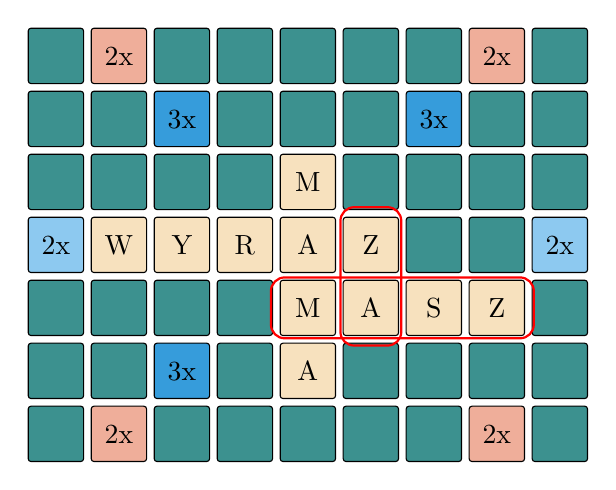
\begin{tikzpicture}
			\tikzstyle{every node}=[draw, shape=rectangle, rounded corners = 1pt, minimum width = 20pt, minimum height = 20pt, align=center, text height = 7pt];
			\node [fill=Board] at (-0.8, 0) {};
			\node [fill=DoubleWordBonus] at (0, 0) {2x};
			\node [fill=Board] at (0.8, 0) {};
			\node [fill=Board] at (1.6, 0) {};
			\node [fill=Board] at (2.4, 0) {};
			\node [fill=Board] at (3.2, 0) {};
			\node [fill=Board] at (4.0, 0) {};
			\node [fill=DoubleWordBonus] at (4.8, 0) {2x};
			\node [fill=Board] at (5.6, 0) {};
			\node [fill=Board] at (-.8, -.8) {};
			\node [fill=Board] at (0, -.8) {};
			\node [fill=TripleLetterBonus] at (0.8, -.8) {3x};
			\node [fill=Board] at (1.6, -.8) {};
			\node [fill=Board] at (2.4, -.8) {};
			\node [fill=Board] at (3.2, -.8) {};
			\node [fill=TripleLetterBonus] at (4.0, -.8) {3x};
			\node [fill=Board] at (4.8, -.8) {};
			\node [fill=Board] at (5.6, -.8) {};
			\node [fill=Board] at (-.8, -1.6) {};
			\node [fill=Board] at (0, -1.6) {};
			\node [fill=Board] at (0.8, -1.6) {};
			\node [fill=Board] at (1.6, -1.6) {};
			\node [fill=Tile] at (2.4, -1.6) {M};
			\node [fill=Board] at (3.2, -1.6) {};
			\node [fill=Board] at (4.0, -1.6) {};
			\node [fill=Board] at (4.8, -1.6) {};
			\node [fill=Board] at (5.6, -1.6) {};
			\node [fill=DoubleLetterBonus] at (-.8, -2.4) {2x};
			\node [fill=Tile] at (0, -2.4) {W};
			\node [fill=Tile] at (.8, -2.4) {Y};
			\node [fill=Tile] at (1.6, -2.4) {R};
			\node [fill=Tile] at (2.4, -2.4) {A};
			\node [fill=Tile] at (3.2, -2.4) {Z};
			\node [fill=Board] at (4.0, -2.4) {};
			\node [fill=Board] at (4.8, -2.4) {};
			\node [fill=DoubleLetterBonus] at (5.6, -2.4) {2x};
			\node [fill=Board] at (-.8, -3.2) {};
			\node [fill=Board] at (0, -3.2) {};
			\node [fill=Board] at (0.8, -3.2) {};
			\node [fill=Board] at (1.6, -3.2) {};
			\node [fill=Tile] at (2.4, -3.2) {M};
			\node [fill=Tile] at (3.2, -3.2) {A};
			\node [fill=Tile] at (4.0, -3.2) {S};
			\node [fill=Tile] at (4.8, -3.2) {Z};
			\node [fill=Board] at (5.6, -3.2) {};
			\node [fill=Board] at (-.8, -4.0) {};
			\node [fill=Board] at (0, -4.0) {};
			\node [fill=TripleLetterBonus] at (0.8, -4.0) {3x};
			\node [fill=Board] at (1.6, -4.0) {};
			\node [fill=Tile] at (2.4, -4.0) {A};
			\node [fill=Board] at (3.2, -4.0) {};
			\node [fill=Board] at (4.0, -4.0) {};
			\node [fill=Board] at (4.8, -4.0) {};
			\node [fill=Board] at (5.6, -4.0) {};
			\node [fill=Board] at (-.8, -4.8) {};
			\node [fill=DoubleWordBonus] at (0, -4.8) {2x};
			\node [fill=Board] at (0.8, -4.8) {};
			\node [fill=Board] at (1.6, -4.8) {};
			\node [fill=Board] at (2.4, -4.8) {};
			\node [fill=Board] at (3.2, -4.8) {};
			\node [fill=Board] at (4.0, -4.8) {};
			\node [fill=DoubleWordBonus] at (4.8, -4.8) {2x};
			\node [fill=Board] at (5.6, -4.8) {};
			\node [draw, thick, shape = rectangle, rounded corners = 5pt, color = red, fill = none, minimum height = 22 pt, minimum width = 95 pt] at (3.6, -3.2) {};
			\node [draw, thick, shape = rectangle, rounded corners = 5pt, color = red, fill = none, minimum width = 22 pt, minimum height = 50 pt] at (3.2, -2.8) {};
		\end{tikzpicture}
		\caption{Fragment planszy. Ruch przez dołożenie liter A, S, Z tworzy dwa wyrazy w~układzie krzyżówkowym.}
		\label{fig:crossword_second}
	\end{center}
\end{figure}

W~trakcie jednego ruchu zawodnik może układać płytki tylko w~jednym kierunku (pionowo lub poziomo). Utworzony przez zawodnika wyraz musi być spójny, to znaczy, że wszystkie płytki muszą przylegać do siebie bezpośrednio lub poprzez płytki już istniejące na planszy. Wymagane jest, aby tworzone słowo przylegało do przynajmniej jednej płytki, która jest już umieszczona na planszy (nie dotyczy to pierwszego ruchu).

Punktacja za dane zagranie jest obliczana jako suma punktów za wszystkie płytki, które wchodzą w~skład utworzonych wyrazów (a~więc również tych, które przed zagraniem znajdowały się na planszy), z~uwzględnieniem niewykorzystanych premii wynikających z~pozycji płytki na planszy:

\begin{description}
 \item [Premia literowa] podwaja lub potraja wartość danej płytki.
 \item [Premia słowna] podwaja lub potraja wartość całego wyrazu.
\end{description}

\section*{Strategia optymalna}

Kluczowym zagadnieniem podczas implementacji algorytmu sztucznej inteligencji do gier planszowych (w~tym Scrabble) jest zbadanie istnienia strategii optymalnej.

\begin{theorem}
	Istnieje optymalna strategia gry w~Scrabble.
	\label{thm:optimal_strategy_existence}
\end{theorem}

Aby dowieść twierdzenie \ref{thm:optimal_strategy_existence}~należy uprzednio zdefiniować przestrzeń stanów w~Scrabble.

\begin{definition}
	Stan rozgrywki po danej turze opisują jednoznacznie rozmieszczenie klocków na planszy $P$~oraz zagranie $Z$. Przejście między stanami determinuje zmiana $(\Delta P, \Delta Z)$.
	\label{def:scrabble_state_space}
\end{definition}

Dysponując definicją \ref{def:scrabble_state_space}~można dowieść twierdzenie \ref{thm:optimal_strategy_existence}. Ilustrację dla dowodu \ref{pro:optimal_strategy_existence}~przedstawia rysunek \ref{fig:state_space}.

\begin{pro}
	Dla ułatwienia analiza rozgrywki zostanie przeprowadzona wychodząc od stanu końcowego. Nie wpływa to na ogólność dowodu. Dla dowolnej rozgrywki prawdziwe jest twierdzenie, że do stanu końcowego można wejść tylko na skończoną liczbę sposobów, które reprezentują legalne zagrania. Przeprowadzając rozumowanie iteracyjne możliwe jest przejście do stanu początkowego. Należy zauważyć, że w~każdej iteracji analizowana liczba wejść do stanu jest zawsze skończona, ponieważ skończona jest liczba kombinacji, na które można wylosować litery oraz liczba zagrań legalnych dla danej kombinacji liter. Podobne rozumowanie można przeprowadzić dla każdego stanu końcowego, budując skończone drzewo przestrzeni stanów. Skoro drzewo przestrzeni stanów jest skończone, można na podstawie jego znajomości w~każdym zagraniu wyznaczyć ruch, który maksymalizuje prawdopodobieństwo wygranej.
	\label{pro:optimal_strategy_existence}
\end{pro}

\begin{figure}[ht!]
	\begin{center}
			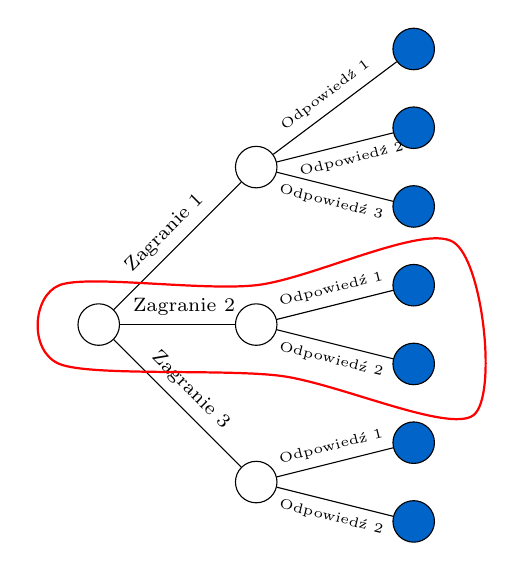
\begin{tikzpicture}
				\tikzstyle{state} = [draw, shape=circle, minimum width=15pt, minimum height=15pt]
				\node (s0) [state] at (0,0) {};
				\node (s1) [state] at (2,2) {};
				\node (s2) [state] at (2,0) {};
				\node (s3) [state] at (2, -2) {};
				\node (s4) [state, fill=UniGreen] at (4,3.5) {};
				\node (s5) [state, fill=UniGreen] at (4,2.5) {};
				\node (s6) [state, fill=UniGreen] at (4,1.5) {};
				\node (s7) [state, fill=UniGreen] at (4,0.5) {};
				\node (s8) [state, fill=UniGreen] at (4,-0.5) {};
				\node (s9) [state, fill=UniGreen] at (4,-1.5) {};
				\node (s10) [state, fill=UniGreen] at (4,-2.5) {};
				\draw (s0) -- node[above, sloped, font=\scriptsize] {Zagranie 1} (s1);
				\draw (s0) -- node[above, sloped, font=\scriptsize, near end, xshift=-8pt] {Zagranie 2} (s2);
				\draw (s0) -- node[above, sloped, font=\scriptsize] {Zagranie 3} (s3);
				\draw (s1) -- node[above, sloped, font=\tiny] {Odpowiedź 1} (s4);
				\draw (s1) -- node[xshift=-6pt, below, near end, sloped, font=\tiny] {Odpowiedź 2} (s5);
				\draw (s1) -- node[below, sloped, font=\tiny] {Odpowiedź 3} (s6);
				\draw (s2) -- node[above, sloped, font=\tiny] {Odpowiedź 1} (s7);
				\draw (s2) -- node[below, sloped, font=\tiny] {Odpowiedź 2} (s8);
				\draw (s3) -- node[above, sloped, font=\tiny] {Odpowiedź 1} (s9);
				\draw (s3) -- node[below, sloped, font=\tiny] {Odpowiedź 2} (s10);
				\draw [red, thick] plot [smooth cycle] coordinates {(-0.5, -0.5) (-0.5, 0.5) (2, 0.5) (4.5, 1.05) (4.76, -1.15) (2.3, -0.65)};
			\end{tikzpicture}
			\caption{Ilustracja dowodu istnienia strategii optymalnej. Stany końcowe oznaczono kolorem niebieskim.}
			\label{fig:state_space}
	\end{center}
\end{figure}

Zostało udowodnione, że deterministyczna wersja Scrabble dla dwóch graczy należy do problemów klasy \emph{PSPACE-Complete}. \cite{deterministic_scrabble} Klasa \emph{PSPACE-Complete} jest najbardziej obszerną klasą problemów wielomianowych. Każdy problem należący do przestrzeni problemów wielomianowych można przekształcić, w~wielomianowym czasie, do problemu klasy \emph{PSPACE-Complete}.

\section*{Strategia zależna od fazy gry}

Niestety, w~praktyce wykorzystywanie strategii optymalnej nie jest możliwe. Dla rozgrywki końcowej 7~klocków przeciwko 7~klockom średnia ilość gałęzi w~drzewie przestrzeni stanów wynosi 200. Kolejnym problemem jest głębokość drzewa, która może sięgać czternastu poziomów (gdy gracze wykładają klocki pojedynczo) lub więcej (dochodzi możliwość pasowania). Wartości te są zbyt duże, by stosować pełny algorytm typu $\alpha - \beta$, a~odnoszą się wyłącznie do sytuacji, w~której posiadamy pełną informację o~rozgrywce (to znaczy znane są klocki przeciwnika). Na pozostałych etapach rozgrywki analiza przestrzeni stanów nie jest opcją. Wynika z~tego, że algorytm sztucznej inteligencji do Scrabble musi zmieniać strategię rozgrywki w~zależności od etapu gry.

Wyróżnia się cztery zasadnicze fazy rozgrywki: \cite{sheppard_maven}

\begin{description}
	\item[Opening Play]\footnote{Opening Play, w~skrócie OP. W~dalszej części artykułu dla określenia faz rozgrywki stosowane będą wyłącznie nazwy skrótowe, a~więc OP, MG, PEG oraz EG} faza otwarcia. Dotyczy wyłącznie pierwszego zagrania, a~więc kiedy na planszy nie znajduje się jeszcze żaden klocek.
	\item[Mid Game] faza śródgry. Rozpoczyna się po otwarciu, a~kończy wraz z~rozpoczęciem fazy PEG.
	\item[Pre-End Game] faza przedkońcowa rozgrywki. Rozpoczyna się w~momencie, kiedy rozgrywka może zakończyć się w~dwóch turach, a~więc kiedy w~worku pozostaje siedem lub mniej klocków. Kończy się wraz z~rozpoczęciem fazy EG.
	\item[End Game] faza zakończenia. Rozpoczyna się, gdy w~worku nie ma już klocków i~trwa aż do końca gry. Charakteryzuje się tym, że w~trakcie jej trwania zawodnicy dysponują pełną informacją o~grze, a~więc również o~literach posiadanych przez przeciwnika.
\end{description}

Wykonywany algorytm będzie różny w~zależności od fazy rozgrywki. Podczas implementacji takiego rozwiązania warto wykorzystać wzorzec projektowy Strategia. Strategia to wzorzec, który ,,definiuje rodzinę algorytmów, pakuje je jako osobne klasy i~powoduje, że są one w pełni wymienne. Zastosowanie strategii pozwala na to, aby zmiany w~implementacji przetwarzania były całkowicie niezależne od strony klienta, który z nich korzysta''. \cite{strategy_pattern_definition} Wzorzec strategii dostosowany do opisywanej dziedziny problemu został schematycznie przedstawiony na rysunku \ref{fig:strategy_pattern}.

\begin{figure}[ht!]
	\centering
	\scalebox{0.7}{
		\begin{tikzpicture}
			\tikzumlset{fill class=white!100}
			\umlclass[type=interface,x=0,y=4]{ScrabbleAI}{\# phase : GamePhase}{+ move() : void \\ \# pickStrategy() : IMoveStrategy} 
			\umlclass[type=interface,x=0,y=0]{IMoveStrategy}{}{+ move() : void} 
			\umlclass[x=-3, y=-3]{FirstPlayStrategy}{}{+ move() : void}
			\umlclass[x=0, y=-6]{MidGameStrategy}{}{+ move() : void}
			\umlclass[x=3, y=-3]{EndGameStrategy}{}{+ move() : void}
			\umluniassoc{ScrabbleAI}{IMoveStrategy}
			\umlimpl{IMoveStrategy}{FirstPlayStrategy}
			\umlimpl{IMoveStrategy}{MidGameStrategy}
			\umlimpl{IMoveStrategy}{EndGameStrategy}
		\end{tikzpicture}
	}
	\caption{Przykład użycia wzorca projektowego Strategia w~kontekście implementacji algorytmu.}
	\label{fig:strategy_pattern}
\end{figure}

\section*{Opening Play}

Celem fazy OP jest wybranie najwyżej punktowanego zagrania. W~algorytmie Quackle wybór ten jest dokonywany poprzez przeszukiwanie słownika pod kątem posiadanych liter. Wynik punktowy uzyskany za zagranie jest obliczany dynamicznie. 

Wyszukiwanie najlepszego otwarcia może być zoptymalizowane czasowo. Wykorzystując znajomość słownika można przeprowadzić analizę najlepszych otwarć dla wszystkich możliwych kombinacji klocków. Każdej kombinacji liter można przypisać prostą funkcję skrótu, która sortuje te litery alfabetycznie. Po wstępnej analizie słownika można przygotować mapę, która każdej funkcji skrótu przyporządkuje najlepsze zagranie oraz jego wartość punktową. Dzięki temu możliwe jest wykonanie pierwszego zagrania w~czasie jednostkowym\footnote{Przy założeniu, że wśród liter początkowych nie znajdują się blanki.}.

\section*{Mid Game}

W~fazie MG w~aplikacji Quackle wykorzystywany jest algorytm z~heurystyczną funkcją statyczną oraz symulacją dwóch zagrań w~przyszłość. Schemat tego algorytmu został przedstawiony na rysunku \ref{fig:mid_game_algorithm}.~\cite{quackle_algorithm}

\begin{figure}[ht!]
	\centering
	\scalebox{0.57}{
		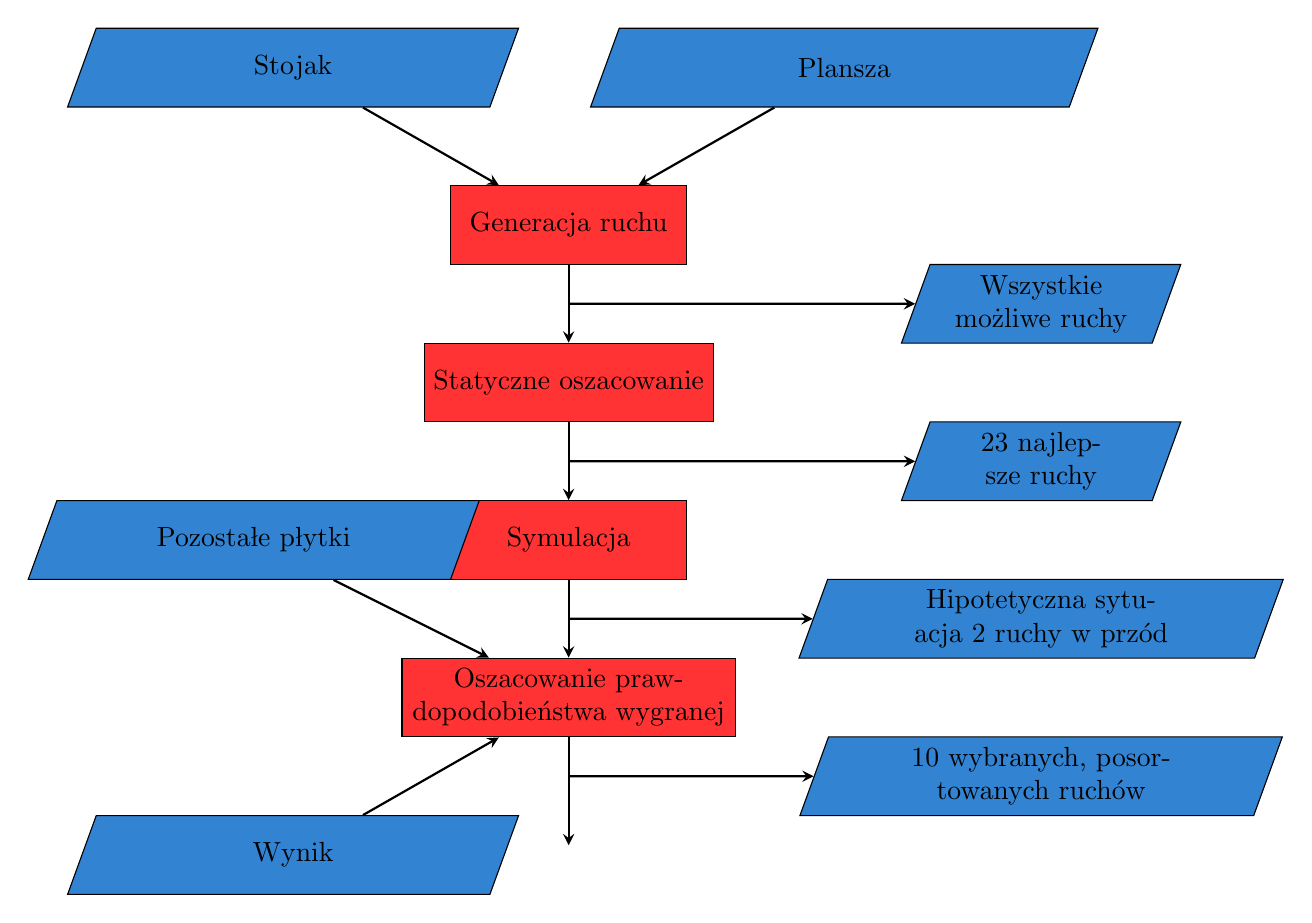
\begin{tikzpicture}[node distance=2cm]
			\noindent
			\tikzstyle{io} = [trapezium, trapezium left angle=70, trapezium right angle=110, minimum width=2cm, minimum height=1cm, text centered, draw=black, fill=UniGreen!80, text width=2.5cm]
			\tikzstyle{process} = [rectangle, minimum width=3cm, minimum height=1cm, text centered, draw=black, fill=red!80]
			\tikzstyle{arrow} = [thick,->,>=stealth]
					
			\node (rack) [io] {Stojak};
			\node (board) [io, right of=rack, xshift=5cm] {Plansza};
			\coordinate (rackboard) at ($(rack)!0.5!(board)$);
			\node (movegen) [process, below of= rackboard] {Generacja ruchu};
			\node (staticeval) [process, below of=movegen] {Statyczne oszacowanie};
			\coordinate (movegenstaticeval) at ($(movegen)!0.5!(staticeval)$);
			\node (possmoves) [io, right of=movegenstaticeval, xshift=4cm] {Wszystkie możliwe ruchy};
			\node (simulation) [process, below of=staticeval] {Symulacja};
			\node (bestmoves) [io, below of=possmoves] {23 najlepsze ruchy};
			\node (hypsequences) [io, below of=bestmoves, text width=5cm] {Hipotetyczna sytuacja 2 ruchy w~przód};
			\node (winpercestimation) [process, below of=simulation, text width=4cm] {Oszacowanie prawdopodobieństwa wygranej};
			\node (end) [process, draw=none, fill=none, below of=winpercestimation, minimum height=1mm] { };
			\coordinate (staticevalsimulation) at ($(staticeval)!0.5!(simulation)$);
			\node (tilesleft) [io, left of=winpercestimation,xshift=-2cm,yshift=2cm] {Pozostałe płytki};
			\node (score) [io, left of=winpercestimation,xshift=-1.5cm,yshift=-2cm] {Wynik};
			\coordinate (winpercestimationend) at ($(winpercestimation)!0.5!(end)$);
			\node (chosenmoves) [io, below of=hypsequences,text width=5cm] {10 wybranych, posortowanych ruchów};
			\draw [arrow] (movegen) -- (staticeval);
			\draw [arrow] (staticeval) -- (simulation);
			\draw [arrow] (simulation) -- (winpercestimation);
			\draw [arrow] (rack) -- (movegen);
			\draw [arrow] (board) -- (movegen);
			\draw [arrow] (winpercestimation) -- (end);
			\draw [arrow] (tilesleft) -- (winpercestimation);
			\draw [arrow] (score) -- (winpercestimation);
			\draw [arrow] ($(movegen)!0.5!(staticeval)$) -- (possmoves);
			\draw [arrow] ($(staticeval)!0.5!(simulation)$) -- (bestmoves);
			\draw [arrow] ($(simulation)!0.5!(winpercestimation)$) -- (hypsequences);
			\draw [arrow] ($(winpercestimation)!0.5!(end)$) -- (chosenmoves);
		\end{tikzpicture}
	}
	\caption{Schemat algorytmu dla fazy MG.}
	\label{fig:mid_game_algorithm}
\end{figure}

Algorytm składa się z~czterech kroków:

\begin{enumerate}
	\item Na podstawie stanu planszy i~dostępnych klocków generowane są wszystkie możliwości ruchu.
	\item Dla każdej możliwości ruchu obliczana jest funkcja oszacowania. Ruchy są sortowane względem malejącej wartości funkcji oszacowania. Lista ruchów jest skracana do najlepszych 23 pozycji.
	\item Dla każdego z~pozostałych ruchów wykonywana jest symulacja stanu rozgrywki na dwa kroki w~przód.
	\item Dla każdego rezultatu oszacowania, biorąc pod uwagę liczbę płytek pozostałych do końca rozgrywki, obliczane jest prawdopodobieństwo wygranej. W~rezultacie powstaje lista 10 ruchów o~największym oszacowanym prawdopodobieństwie wygranej.
\end{enumerate}

\section*{Słowniki do gier}

Reguły Scrabble dopuszczają układanie ,,wszystkich słów występujących w~słownikach języka polskiego oraz wszystkich ich prawidłowych form gramatycznych, z~wyjątkiem takich słów, które rozpoczynają się od wielkiej litery, są skrótami, bądź słowami wymagającymi cudzysłowu lub łącznika''. \cite{scrabble_word_rules} 

Brak zamkniętej listy słów możliwych do wykorzystania w~grze prowadzi do konfliktu interesów, ponieważ gracze sami muszą rozstrzygnąć między sobą, czy dany wyraz jest dopuszczalny, czy nie. Aby umożliwić uczciwą rozgrywkę konieczne było stworzenie zbioru, który zawiera listę słów, wraz ze wszystkimi poprawnymi odmianami, dopuszczalnych do wykorzystania w~grach słownych. W~taki sposób zaczęły powstawać słowniki wyrazów do gier. \cite{game_dictionary_definition}

W~chwili obecnej istnieją dwa duże polskie słowniki do gier:

\begin{description}
 \item [Oficjalny Słownik Polskiego Scrabblisty] Przygotowany przez wydawnictwo naukowe PWN. Dopuszcza użycie wyrazów znajdujących się w~słownikach PWN wydanych po roku 1980.
 \item[Słownik alternatywny] Przygotowany na potrzeby serwisu z~grami internetowymi \url{http://kurnik.pl}. Jest rozwijany przez administratorów serwisu przy współpracy z~internautami. Dopuszcza użycie wyrazów znajdujących się w~słownikach dowolnego wydawnictwa wydanych po roku 1980, z~wyłączeniem czarnej listy słowników\footnote{Jest to lista słowników, które nie zostały dopuszczone jako źródło wyrazów ze względu na niedostateczną jakość opracowania.}. 
\end{description}

Poza dopuszczalnymi źródłami informacji słowniki posiadają jeszcze jedną znaczącą różnicę. Oficjalny Słownik Polskiego Scrabblisty jest dystrybuowany jako program umieszczony na płycie CD, który nie udostępnia listy wszystkich wyrazów zawartych w~słowniku. Program pozwala jedynie sprawdzić, czy dane słowo jest dopuszczalne. Słownik alternatywny dostępny jest w Internecie również w~postaci listy wszystkich dopuszczalnych wyrazów zebranych w~pliku tekstowym. Pozwala to na przeprowadzenie analiz statystycznych, stąd w~dalszej części artykułu autor rozważa wyłącznie Słownik alternatywny.

\section*{Analiza statystyczna}

W~celu wyznaczenia heurystyk mogących wspomóc sztuczną inteligencję grającą w~Scrabble autor przeanalizował dane zawarte w~Słowniku alternatywnym. Pierwszą analizowaną informacją jest częstotliwość występowania poszczególnych liter w~słowniku. Wynika to z~faktu, że zasady gry Scrabble są oparte na rozkładzie prawdopodobieństwa występowania liter w~danym języku. Możliwe jest, że badanie statystyczne słownika przyniesie informacje o~literach, których warto używać w~pierwszej kolejności.

Wykres przedstawiony na rysunku 69 dostarcza nam informacji, że autorzy polskich reguł do gry Scrabble nie oszacowali poprawnie częstotliwości występowania wszystkich liter. Przykładowo litera \textbf{o} występuje w~słowniku częściej niż litera \textbf{e}, natomiast prawdopodobieństwo wylosowania odpowiadających tym literom płytek w~grze kształtuje się odwrotnie. Wynika z~tego, że porównując dwa podobnie punktowane zagrania, warto wybrać to, które wykorzystuje więcej samogłosek \textbf{e} niż \textbf{o}. Podobną zależność można stwierdzić w~przypadku litery \textbf{h}, której częstotliwość występowania została przez autorów zasad znacząco zawyżona. Korzytnie jest wybierać zagrania, które powodują wyłożenie płytek z~literą \textbf{h}.

Interesującą statystyką są najlepsze otwarcia (czyli pierwsze zagrania w~grze). Pozwalają one, przy wylosowaniu szczęśliwej kombinacji płytek, zagrać w~najbardziej opłacalny sposób (na początku rozgrywki nie ma ryzyka pozostawienia przeciwnikowi ,,otwartej gry''). Statystyka ta jest szczególnie przydatna dla ludzi, chociaż również sztuczna inteligencja może wykorzystać ją do pominięcia zbędnych obliczeń. Najlepsze otwarcia dla słownika alternatywnego zebrano na rysunku \ref{fig:best_openings}.

\begin{figure}[ht!]
	\begin{center}
			\begin{tikzpicture}
		\tikzstyle{every node}=[draw, shape=rectangle, rounded corners = 1pt, minimum width = 16pt, minimum height = 16pt, align=center, text height = 5pt, font=\scriptsize];
		\node [fill=Board] at (0, 0) { };
		\node [fill=Board] at (.6, 0) { };
		\node [fill=DoubleLetterBonus] at (1.2, 0) {x2};
		\node [fill=Board] at (1.8, 0) { };
		\node [fill=Board] at (2.4, 0) { };
		\node [fill=Board] at (3, 0) { };
		\node [fill=DoubleWordBonus] at (3.6, 0) { };
		\node [fill=Board] at (4.2, 0) { };
		\node [fill=Board] at (4.8, 0) { };
		\node [fill=Board] at (5.4, 0) { };
		\node [fill=DoubleLetterBonus] at (6, 0) {x2};
		\node [fill=Board] at (6.6, 0) { };
		\node [fill=Board] at (7.2, 0) { };		
		\node [shape=star, star points=8, rounded corners = 0pt, fill=black, text height = 0pt] at (3.6, 0) {};
		\node [fill=Tile] at (0, -.6) {P};
		\node [fill=Tile] at (.6, -.6) {Ó};
		\node [fill=Tile] at (1.2, -.6) {Ź};
		\node [fill=Tile] at (1.8, -.6) {N};
		\node [fill=Tile] at (2.4, -.6) {O};
		\node [fill=Tile] at (3, -.6) {Ś};
		\node [fill=Tile] at (3.6, -.6) {Ć};
		\node [fill=Board] at (4.2, -.6) { };
		\node [fill=Board] at (4.8, -.6) { };
		\node [fill=Board] at (5.4, -.6) { };
		\node [fill=DoubleLetterBonus] at (6, -.6) {x2};
		\node [fill=Board] at (6.6, -.6) { };
		\node [fill=Board] at (7.2, -.6) { };	
		\node [fill=Board] at (0, -1.2) { };
		\node [fill=Board] at (.6, -1.2) { };
		\node [fill=DoubleLetterBonus] at (1.2, -1.2) {x2};
		\node [fill=Board] at (1.8, -1.2) { };
		\node [fill=Board] at (2.4, -1.2) { };
		\node [fill=Board] at (3, -1.2) { };
		\node [fill=Tile] at (3.6, -1.2) {B};
		\node [fill=Tile] at (4.2, -1.2) {Ł};
		\node [fill=Tile] at (4.8, -1.2) {Ą};
		\node [fill=Tile] at (5.4, -1.2) {D};
		\node [fill=Tile] at (6, -1.2) {Ź};
		\node [fill=Tile] at (6.6, -1.2) {Ż};
		\node [fill=Tile] at (7.2, -1.2) {E};
		\node [fill=Board] at (0, -1.8) { };
		\node [fill=Board] at (.6, -1.8) { };
		\node [fill=DoubleLetterBonus] at (1.2, -1.8) {x2};
		\node [fill=Board] at (1.8, -1.8) { };
		\node [fill=Board] at (2.4, -1.8) { };
		\node [fill=Board] at (3, -1.8) { };
		\node [fill=Tile] at (3.6, -1.8) {U};
		\node [fill=Tile] at (4.2, -1.8) {B};
		\node [fill=Tile] at (4.8, -1.8) {O};
		\node [fill=Tile] at (5.4, -1.8) {D};
		\node [fill=Tile] at (6, -1.8) {Ź};
		\node [fill=Tile] at (6.6, -1.8) {Ż};
		\node [fill=Tile] at (7.2, -1.8) {E};
		\node [fill=Board] at (0, -2.4) { };
		\node [fill=Board] at (.6, -2.4) { };
		\node [fill=DoubleLetterBonus] at (1.2, -2.4) {x2};
		\node [fill=Board] at (1.8, -2.4) { };
		\node [fill=Board] at (2.4, -2.4) { };
		\node [fill=Board] at (3, -2.4) { };
		\node [fill=Tile] at (3.6, -2.4) {P};
		\node [fill=Tile] at (4.2, -2.4) {Ó};
		\node [fill=Tile] at (4.8, -2.4) {J};
		\node [fill=Tile] at (5.4, -2.4) {D};
		\node [fill=Tile] at (6, -2.4) {Ź};
		\node [fill=Tile] at (6.6, -2.4) {K};
		\node [fill=Tile] at (7.2, -2.4) {Ę};		
		\node [fill=Board] at (0, -3) { };
		\node [fill=Board] at (.6, -3) { };
		\node [fill=DoubleLetterBonus] at (1.2, -3) {x2};
		\node [fill=Board] at (1.8, -3) { };
		\node [fill=Board] at (2.4, -3) { };
		\node [fill=Board] at (3, -3) { };
		\node [fill=Tile] at (3.6, -3) {G};
		\node [fill=Tile] at (4.2, -3) {Ł};
		\node [fill=Tile] at (4.8, -3) {Ó};
		\node [fill=Tile] at (5.4, -3) {D};
		\node [fill=Tile] at (6, -3) {Ź};
		\node [fill=Tile] at (6.6, -3) {Ż};
		\node [fill=Tile] at (7.2, -3) {E};	
		\node [fill=Board] at (0, -3.6) { };
		\node [fill=Board] at (.6, -3.6) { };
		\node [fill=DoubleLetterBonus] at (1.2, -3.6) {x2};
		\node [fill=Board] at (1.8, -3.6) { };
		\node [fill=Board] at (2.4, -3.6) { };
		\node [fill=Board] at (3, -3.6) { };
		\node [fill=Tile] at (3.6, -3.6) {U};
		\node [fill=Tile] at (4.2, -3.6) {B};
		\node [fill=Tile] at (4.8, -3.6) {Ą};
		\node [fill=Tile] at (5.4, -3.6) {D};
		\node [fill=Tile] at (6, -3.6) {Ź};
		\node [fill=Tile] at (6.6, -3.6) {Ż};
		\node [fill=Tile] at (7.2, -3.6) {E};		
		\node [fill=Board] at (0, -4.2) { };
		\node [fill=Board] at (.6, -4.2) { };
		\node [fill=DoubleLetterBonus] at (1.2, -4.2) {x2};
		\node [fill=Board] at (1.8, -4.2) { };
		\node [fill=Board] at (2.4, -4.2) { };
		\node [fill=Board] at (3, -4.2) { };
		\node [fill=Tile] at (3.6, -4.2) {U};
		\node [fill=Tile] at (4.2, -4.2) {G};
		\node [fill=Tile] at (4.8, -4.2) {Ó};
		\node [fill=Tile] at (5.4, -4.2) {D};
		\node [fill=Tile] at (6, -4.2) {Ź};
		\node [fill=Tile] at (6.6, -4.2) {Ż};
		\node [fill=Tile] at (7.2, -4.2) {E};		
		\node [fill=Board] at (0, -4.8) { };
		\node [fill=Board] at (.6, -4.8) { };
		\node [fill=DoubleLetterBonus] at (1.2, -4.8) {x2};
		\node [fill=Board] at (1.8, -4.8) { };
		\node [fill=Board] at (2.4, -4.8) { };
		\node [fill=Board] at (3, -4.8) { };
		\node [fill=Tile] at (3.6, -4.8) {B};
		\node [fill=Tile] at (4.2, -4.8) {L};
		\node [fill=Tile] at (4.8, -4.8) {U};
		\node [fill=Tile] at (5.4, -4.8) {Ź};
		\node [fill=Tile] at (6, -4.8) {Ń};
		\node [fill=Tile] at (6.6, -4.8) {Ż};
		\node [fill=Tile] at (7.2, -4.8) {E};	
		\node [fill=Board] at (0, -5.4) { };
		\node [fill=Board] at (.6, -5.4) { };
		\node [fill=DoubleLetterBonus] at (1.2, -5.4) {x2};
		\node [fill=Board] at (1.8, -5.4) { };
		\node [fill=Board] at (2.4, -5.4) { };
		\node [fill=Board] at (3, -5.4) { };
		\node [fill=Tile] at (3.6, -5.4) {P};
		\node [fill=Tile] at (4.2, -5.4) {Ó};
		\node [fill=Tile] at (4.8, -5.4) {J};
		\node [fill=Tile] at (5.4, -5.4) {D};
		\node [fill=Tile] at (6, -5.4) {Ź};
		\node [fill=Tile] at (6.6, -5.4) {K};
		\node [fill=Tile] at (7.2, -5.4) {Ą};		
		\node [fill=Board] at (0, -6) { };
		\node [fill=Board] at (.6, -6) { };
		\node [fill=DoubleLetterBonus] at (1.2, -6) {x2};
		\node [fill=Board] at (1.8, -6) { };
		\node [fill=Board] at (2.4, -6) { };
		\node [fill=Tile] at (3, -6) {U};
		\node [fill=Tile] at (3.6, -6) {G};
		\node [fill=Tile] at (4.2, -6) {R};
		\node [fill=Tile] at (4.8, -6) {Z};
		\node [fill=Tile] at (5.4, -6) {Ą};
		\node [fill=Tile] at (6, -6) {Ź};
		\node [fill=Tile] at (6.6, -6) {Ć};
		\node [fill=Board] at (7.2, -6) { };		
	\end{tikzpicture}
	\caption{Najlepsze otwarcia dla Słownika alternatywnego. Słowo \emph{późność} jest warte 126 punktów, pozostałe po 124 punkty.}
	\label{fig:best_openings}
	\end{center}
\end{figure}

Dokonując statystycznej analizy słownika warto wziąć pod uwagę najbardziej opłacalne kombinacje liter. W~trakcie rozgrywki gracze dążą do układania wyrazów, które wymagają użycia wszystkich siedmiu płytek znajdujących się na stojaku. Zagranie takie jest bowiem nagradzane dodatkową premią w~wysokości 50 punktów. Stąd przez najbardziej opłacalną kombinację liter należy rozumieć taką zawartość stojaka, która pozwala ułożyć jak najwięcej wyrazów siedmioliterowych. Duża liczba kombinacji sprawia, że z~większym prawdopodobieństwem uda nam się dopasować wyraz do istniejącego układu płytek na planszy. Autor przeanalizował najlepsze kombinacje liter dla Słownika alternatywnego. Wyniki zebrane są w~tabeli \ref{tab:best_letter_combos}.

\begin{figure}[ht!]
	\begin{center}
				\scalebox{0.9}{
				\begin{tabular}{|c|c|}
					\hline
					Litery	&	Liczba możliwych do	 \\
					& ułożenia wyrazów \\
					\hline
					E, I, K, L, N, O, W	&	12 słów	\\
					A, E, I, K, P, R, S	&	12 słów	\\
					A, E, I, K, L, N, P	&	12 słów	\\
					A, E, K, N, R, T, Y	&	11 słów	\\
					A, I, K, M, O, P, S&	11 słów	\\
					A, I, K, M, O, R, W&	11 słów	\\
					A, A, I, K, L, M, S	&	10 słów	\\
					A, I, K, M, O, S, T&	10 słów	\\
					A, I, K, L, N, O, W	&	10 słów	\\
					A, I, K, L, M, N, O&	10 słów	\\
					\hline
				\end{tabular}
				}
			\caption{Najlepsze kombinacje liter dla Słownika alternatywnego.}
			\label{tab:best_letter_combos}
	\end{center}
\end{figure}

Najbardziej opłacalne kombinacje liter można wykorzystać do strategicznego planowania zagrań. Wykonując poszczególne ruchy korzystnie jest dążyć do uzyskania jednego z~przedstawionych układów liter na stojaku. Można tego dokonać poprzez usuwanie płytek, które nie zostały uwzględnione w~tych kombinacjach, jak również usuwanie płytek zduplikowanych (częstą sytuacją jest posiadanie kilku płytek z~tą samą samogłoską).

\section*{Wyznaczanie wszystkich dopuszczalnych ruchów}

Podstawowym zadaniem sztucznej inteligencji w~grze Scrabble jest wyznaczenie (na podstawie zadanego słownika) wszystkich dopuszczalnych ruchów w~danej turze. Odpowiedni algorytm został opracowany przez A.~Appela i~G.~Jacobsona. \cite{worlds_fastest_scrabble_program} Autorzy proponują opisanie słownika za pomocą grafowej stuktury o~nazwie DAWG\footnote{Z~angielskiego Directed Acyclic Word Graph - skierowany, niecykliczny graf słów.}. Jest to odmiana drzewa trie\footnote{Od angielskiego słowa \emph{retrieval}, które oznacza odczyt.}, która charakteryzuje się silną kompresją danych uzyskiwaną dzięki łączeniu krawędziami identycznych sufiksów wyrazów. Przykładowy słownik DAWG został przedstawiony na rysunku \ref{fig:dawg_example}.

\begin{figure}[ht!]
	\begin{center}
			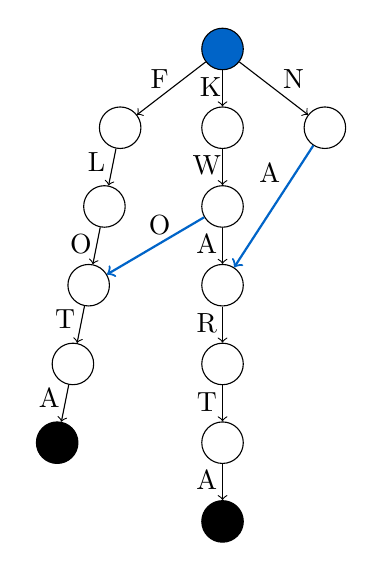
\begin{tikzpicture}
				\tikzstyle{every node}=[draw, shape=circle, minimum width = 15pt, minimum height = 15pt, text height = 0pt];
				\node [fill=UniGreen] (root) at (0,0) {};
				\node (n01) at (-1.3,-1) {};
				\node (n02) at (0, -1) {};
				\node (n03) at (1.3, -1) {};
				\node [draw=none] (t01) at (-0.8, -0.5) {F};
				\node [draw=none] (t02) at (-0.15, -0.6) {K};
				\node [draw=none] (t01) at (0.9, -0.5) {N};
				\draw[->] (root) -- (n01);
				\draw[->] (root) -- (n02);
				\draw[->] (root) -- (n03);
				\node (n11) at (-1.5, -2) {};
				\node (n12) at (0, -2) {};
				\node [draw=none] (t11) at (-1.6, -1.55) {L};
				\node [draw=none] (t12) at (-0.2, -1.6) {W};
				\node [draw=none] (t23) at (0.6, -1.7) {A};
				\draw[->] (n01) -- (n11);
				\draw[->] (n02) -- (n12);
				\node (n21) at (-1.7, -3) {};
				\node (n22) at (0, -3) {};
				\node [draw=none] (t21) at (-1.8, -2.6) {O};
				\node [draw=none] (t22) at (-0.8, -2.35) {O};
				\node [draw=none] (t23) at (-0.2, -2.6) {A};
				\draw[->] (n11) -- (n21);
				\draw[->, color=UniGreen, thick] (n12) -- (n21);
				\draw[->] (n12) -- (n22);
				\draw[->, color=UniGreen, thick] (n03) -- (n22);
				\node (n31) at (-1.9, -4) {};
				\node (n32) at (0, -4) {};
				\node [draw=none] (t31) at (-2.0, -3.55) {T};
				\node [draw=none] (t32) at (-0.2, -3.6) {R};
				\draw[->] (n21) -- (n31);
				\draw[->] (n22) -- (n32);
				\node [fill=black] (n41) at (-2.1, -5) {};
				\node (n42) at (0, -5) {};
				\node [draw=none] (t41) at (-2.2, -4.55) {A};
				\node [draw=none] (t42) at (-0.2, -4.6) {T};
				\draw[->] (n31) -- (n41);
				\draw[->] (n32) -- (n42);
				\node [fill=black] (n51) at (0, -6) {};
				\node [draw=none] (t51) at (-0.2, -5.6) {A};
				\draw[->] (n42) -- (n51);
			\end{tikzpicture}
			\caption{Struktura DAWG, która opisuje wyrazy \emph{flota}, \emph{kwota}, \emph{kwarta} oraz \emph{narta}.}
			\label{fig:dawg_example}
	\end{center}
\end{figure}

Autorzy wybrali tę strukturę ze względu na bardzo szybkie wyszukiwanie słów po ich prefiksie, a~także na dobry współczynnik kompresji słownika. Pełen słownik do gier dla języka angielskiego opisany przy pomocy DAWG zajmuje około $2.5$ MB pamięci.

Autorzy przedstawili czterokrokowy algorytm (zwany dalej algorytmem Appela-Jacobsona) wykorzystujący słownik DAWG, który umożliwia wyznaczenie wszystkich możliwych ruchów przy danym stanie planszy i~dostępnych do wykorzystania literach:

\begin{enumerate}
 \item Redukcja złożoności problemu do jednego wymiaru. Algorytm rozpatruje ruchy wyłącznie w~jednym kierunku (pionowo lub poziomo), ograniczając się do jednego wiersza lub kolumny. Rozumowanie to jest powtarzane dla każdego wiersza (lub kolumny), a~następnie plansza do gry jest transponowana i~algorytm wykonywany jest dla drugiego kierunku. W~dalszym opisie autor artykułu zakłada, że rozpatrujemy wyłącznie wiersze, a~nie kolumny, planszy.
 \item Ograniczanie zbioru znaków, które można legalnie wstawić w~daną komórkę. W~tym kroku wykorzystuje się fakt, że tworzenie wyrazów w~danym kierunku może skutkować utworzeniem nowych słów w~kierunku przeciwnym, ale tylko poprzez dodanie jednego znaku. Jest to trywialny do sprawdzenia przypadek, który znacząco ogranicza liczbę możliwych do wykonania legalnych ruchów.
 \item Wyznaczenie kotwic\footnote{W~oryginalnej pracy termin ten został wprowadzony przy pomocy angielskiego zwrotu \emph{anchor}.}. Kotwica jest to najbardziej wysunięta na lewo płytka nowego wyrazu, która przylega do innej, znajdującej się na planszy płytki. Zgodnie z~zasadami gry w~Scrabble, każdy nowo utworzony wyraz musi posiadać dokładnie jedną kotwicę.
 \item Rozwijanie możliwych do utworzenia wyrazów poprzez wyjście od wyznaczonych w~punkcie trzecim kotwic, a~także uwzględnienie wyznaczonych w~punkcie drugim ograniczeń. 
\end{enumerate}

Rozwijanie możliwych wyrazów rozpoczyna się od płytek znajdujących się po lewej stronie kotwicy. Rozpatrywane są trzy przypadki:

\begin{itemize}
 \item Trywialny - na lewo od kotwicy nie ma żadnych płytek.
 \item Trywialny - część wyrazu na lewo od kotwicy składa się wyłącznie z~płytek znajdujących się już na planszy.
 \item Lewa część wyrazu składa się z~liter znajdujących się na stojaku i~dostępnych do zagrania. Należy zbadać wszystkie możliwe kombinacje.
\end{itemize}

Następnie rozwijana jest prawa część wyrazu, która uwzględnia kotwicę oraz wszystkie płytki na prawo od niej. W~tym celu wyszukuje się w~słowniku poprawne sufiksy, które składają się z~dostępnych na stojaku liter oraz spełniają wyznaczone ograniczenia.

Algorytm Appela-Jacobsona jest wydajny, posiada jednak narzut obliczeniowy związany z~wyznaczaniem lewostronnych dopełnień wyrazów. Zakładając, że kotwica jest również ostatnią literą nowego wyrazu, należy zbadać $6! = 720$ lewostronnych kombinacji. W~pesymistycznym przypadku, kiedy na stojaku znajdują się dwa blanki\footnote{Blank - płytka, która nie posiada wartości punktowej, ale może być zastąpiona dowolną literą.}, liczba badanych kombinacji wzrasta do $\frac{4! \times 32^{2}}{2} = 12288$. Biorąc pod uwagę fakt, że większość wyznaczonych prefiksów w~ogóle nie będzie występować w~słowniku, jest to znaczący narzut.

Powyższa obserwacja stała się podstawą zmodyfikowanego algorytmu zaprezentowanego przez Stevena Gordona. \cite{faster_move_generation_algorithm} Autor nie zmienia kroków algorytmu wykorzystywanych do generacji wszystkich kombinacji ruchów. Zaproponowana modyfikacja obejmuje wykorzystanie struktury GADDAG\footnote{Autor nie podaje rozwinięcia tego skrótu, jednak ze względu na postać przechowywanych w~strukturze danych można domyślać się, że jest ona wariacją nazwy DAG (z~angielskiego Directed Acyclic Graph - skierowany, acykliczny graf).}, w~miejsce słownika DAWG. 

GADDAG jest odmianą drzewa trie, która jest nastawiona na szybkie prefiksowanie wyrazów. Każdy opisany wyraz podzielony jest na dwie części: prefiks oraz sufiks. Wychodząc od korzenia drzewa kolejne wierzchołki opisują prefiks wyrazu czytany od tyłu. Dalej występuje znak zakończenia prefiksu (oznaczany $\gg$), a~następnie sufiks wyrazu czytany w~normalnej kolejności. Kształt struktury jest silnie powiązany z~algorytmem Appela-Jacobsona. Wychodząc od kotwicy w~kierunku lewej strony wyrazu analizowane są kolejne litery prefiksu w~odwróconej kolejności. Dalej następuje przejście do kotwicy i~rozpatrywany jest sufiks w~normalnej kolejności. Ilustruje to rysunek \ref{fig:gaddag_basis}. 

\begin{figure}[ht!]
	\begin{center}
			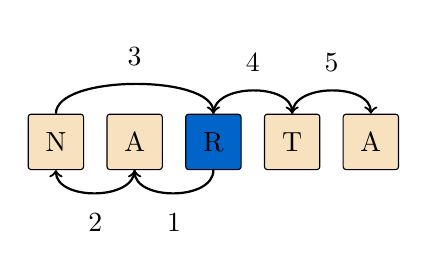
\begin{tikzpicture}
			\tikzstyle{every node}=[draw, shape=rectangle, rounded corners = 1pt, minimum width = 20pt, minimum height = 20pt, align=center, text height = 7pt];
			\node [fill=Tile] (n) at (0, 0) {N};
			\node [fill=Tile] (a1) at (1.0, 0) {A};
			\node [fill=UniGreen] (r) at (2.0, 0) {R};
			\node [fill=Tile] (t) at (3.0, 0) {T};
			\node [fill=Tile] (a2) at (4.0, 0) {A};
			\path (r) edge[out=270,in=270,->, thick] node[below, draw=none, fill=none]{$1$} (a1);
			\draw (a1) edge[out=270,in=270,->, thick] node[below, draw=none, fill=none]{$2$} (n);
			\draw (n) edge[out=90,in=90,->, thick, distance=0.5cm] node[above, draw=none, fill=none]{$3$} (r);
			\draw (r) edge[out=90,in=90,->, thick] node[above, draw=none, fill=none]{$4$} (t);
			\draw (t) edge[out=90,in=90,->, thick] node[above, draw=none, fill=none]{$5$} (a2);
		\end{tikzpicture}
	\end{center}
	\caption{Kolejność analizowania pól w~algorytmie Appela-Jacobsona. Kotwica oznaczona jest na niebiesko.}
	\label{fig:gaddag_basis}
\end{figure}

Przykładowa struktura GADDAG opisująca wyraz ,,narta'' została zaprezentowana na rysunku \ref{fig:gaddag_example}. Należy zauważyć, że sprawdzenie występowania wyrazu w~słowniku wymaga dodatkowego kroku - słowo należy odwrócić. Dla podanego przykładu sprawdzenie poprawności wyrazu narta wymaga poszukiwania frazy $ATRAN \gg$. 

\begin{figure}[ht!]
	\begin{center}
	\scalebox{0.85}{
			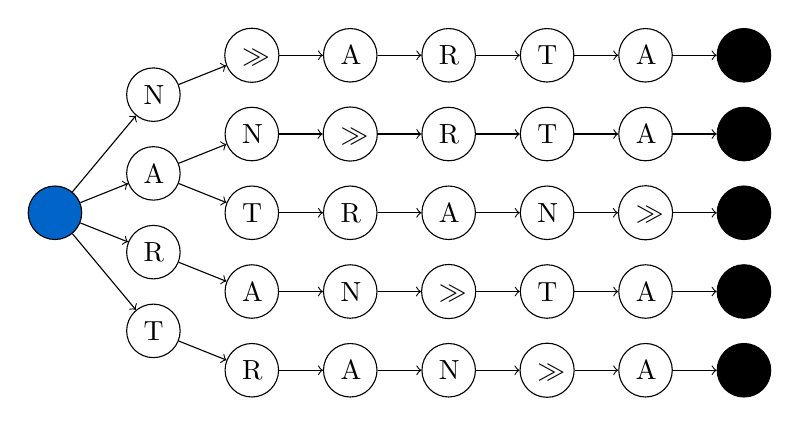
\begin{tikzpicture}
		\tikzstyle{every node}=[draw, shape=circle, minimum width = 15pt, minimum height = 15pt, text height = 7pt, text width = 7pt, align = center];
		\node [fill=UniGreen] (root) at (0,0) {};
		\node (n01) at (1.25, 1.5) {N};
		\node (n02) at (1.25, 0.5) {A};
		\node (n03) at (1.25, -0.5) {R};
		\node (n04) at (1.25, -1.5) {T};
		\node (n11) at (2.5, 2) {$\gg$};
		\node (n12) at (2.5, 1) {N};
		\node (n13) at (2.5, 0) {T};
		\node (n14) at (2.5, -1) {A};
		\node (n15) at (2.5, -2) {R};
		\node (n21) at (3.75, 2) {A};
		\node (n22) at (3.75, 1) {$\gg$};
		\node (n23) at (3.75, 0) {R};
		\node (n24) at (3.75, -1) {N};
		\node (n25) at (3.75, -2) {A};
		\node (n31) at (5, 2) {R};
		\node (n32) at (5, 1) {R};
		\node (n33) at (5, 0) {A};
		\node (n34) at (5, -1) {$\gg$};
		\node (n35) at (5, -2) {N};
		\node (n41) at (6.25, 2) {T};
		\node (n42) at (6.25, 1) {T};
		\node (n43) at (6.25, 0) {N};
		\node (n44) at (6.25, -1) {T};
		\node (n45) at (6.25, -2) {$\gg$};
		\node (n51) at (7.5, 2) {A};
		\node (n52) at (7.5, 1) {A};
		\node (n53) at (7.5, 0) {$\gg$};
		\node (n54) at (7.5, -1) {A};
		\node (n55) at (7.5, -2) {A};
		\node [fill=black] (n61) at (8.75, 2) {};
		\node [fill=black] (n62) at (8.75, 1) {};
		\node [fill=black] (n63) at (8.75, 0) {};
		\node [fill=black] (n64) at (8.75, -1) {};
		\node [fill=black] (n65) at (8.75, -2) {};
		\draw[->] (root) -- (n01);
		\draw[->] (root) -- (n02);
		\draw[->] (root) -- (n03);
		\draw[->] (root) -- (n04);
		\draw[->] (n01) -- (n11);
		\draw[->] (n02) -- (n12);
		\draw[->] (n02) -- (n13);
		\draw[->] (n03) -- (n14);
		\draw[->] (n04) -- (n15);
		\draw[->] (n11) -- (n21);
		\draw[->] (n12) -- (n22);
		\draw[->] (n13) -- (n23);
		\draw[->] (n14) -- (n24);
		\draw[->] (n15) -- (n25);
		\draw[->] (n21) -- (n31);
		\draw[->] (n22) -- (n32);
		\draw[->] (n23) -- (n33);
		\draw[->] (n24) -- (n34);
		\draw[->] (n25) -- (n35);
		\draw[->] (n31) -- (n41);
		\draw[->] (n32) -- (n42);
		\draw[->] (n33) -- (n43);
		\draw[->] (n34) -- (n44);
		\draw[->] (n35) -- (n45);
		\draw[->] (n41) -- (n51);
		\draw[->] (n42) -- (n52);
		\draw[->] (n43) -- (n53);
		\draw[->] (n44) -- (n54);
		\draw[->] (n45) -- (n55);
		\draw[->] (n51) -- (n61);
		\draw[->] (n52) -- (n62);
		\draw[->] (n53) -- (n63);
		\draw[->] (n54) -- (n64);
		\draw[->] (n55) -- (n65);
	\end{tikzpicture}
	}
		\caption{Przykład struktury GADDAG dla wyrazu \emph{narta}.}
		\label{fig:gaddag_example}
	\end{center}
\end{figure}

\section*{Dobór strategii w~zależności od fazy gry}

Rozgrywkę w~Scrabble można podzielić na trzy fazy gry:

\begin{description}
 \item [MG (mid-game)] trwa od rozpoczęcia rozgrywki do rozpoczęcia fazy \emph{PEG},
 \item [PEG (pre-endgame)] rozpoczyna się, kiedy do pobrania pozostają wyłącznie jedna (lub, w~zależności od definicji) dwie płytki,
 \item [EG (end-game)] rozpoczyna się, kiedy nie ma już płytek do pobrania, a~więc gracze znają wzajemnie własne płytki.
\end{description}

W~fazie \emph{MG} liczba możliwych kombinacji płytek przeciwnika oraz ruchów jest tak duża, że nie jest możliwa analiza przestrzeni stanów. Podejściem stosowanym w~tej fazie rozgrywki jest wykorzystanie metod heurystycznych i~symulacji do wyboru najlepszego ruchu. Schemat postępowania zostanie opisany na przykładzie algorytmu wykorzystywanego w~programie \emph{Quackle} - uznawanego za najlepszego komputerowego gracza Scrabble na świecie. \cite{quackle_algorithm} Diagram ilustrujący algorytm został przedstawiony na rysunku \ref{fig:quackle_schema}.

\begin{figure}[ht!]
 	\begin{center}
		\scalebox{0.63}{
			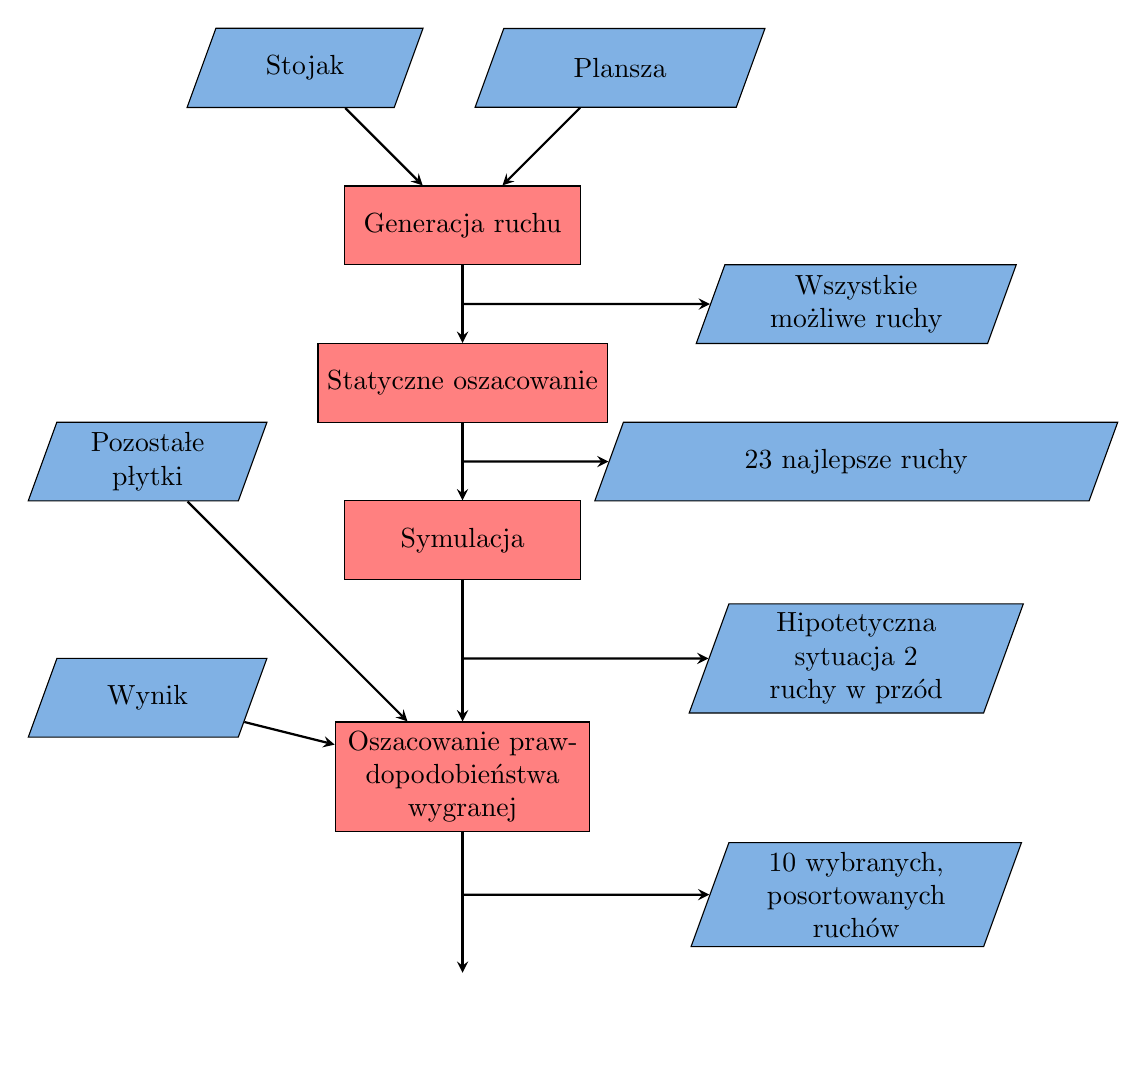
\begin{tikzpicture}[node distance=2cm]
				\tikzstyle{io} = [trapezium, trapezium left angle=70, trapezium right angle=110, minimum width=3cm, minimum height=1cm, text centered, draw=black, fill=UniGreen!50]
				\tikzstyle{process} = [rectangle, minimum width=3cm, minimum height=1cm, text centered, draw=black, fill=red!50]
				\tikzstyle{arrow} = [thick,->,>=stealth]
				
				\node (rack) [io] {Stojak};
				\node (board) [io, right of=rack, xshift=2cm] {Plansza};
				\coordinate (rackboard) at ($(rack)!0.5!(board)$);
				\node (movegen) [process, below of= rackboard] {Generacja ruchu};
				\node (staticeval) [process, below of=movegen] {Statyczne oszacowanie};
				\coordinate (movegenstaticeval) at ($(movegen)!0.5!(staticeval)$);
				\node (possmoves) [io, right of=movegenstaticeval, xshift=3cm, text width=3cm] {Wszystkie możliwe ruchy};
				\node (simulation) [process, below of=staticeval] {Symulacja};
				\node (bestmoves) [io, below of=possmoves, text width=3cm] {23 najlepsze ruchy};
				\node (hypsequences) [io, below of=bestmoves, text width=3cm, yshift=-0.5cm] {Hipotetyczna sytuacja 2 ruchy w~przód};
				\node (winpercestimation) [process, below of=simulation, text width=3cm, yshift=-1cm] {Oszacowanie prawdopodobieństwa wygranej};
				\node (end) [process, draw=none, fill=none, below of=winpercestimation, yshift=-1cm] { };
				\coordinate (staticevalsimulation) at ($(staticeval)!0.5!(simulation)$);
				\node (tilesleft) [io, left of=staticevalsimulation,xshift=-2cm, text width=2cm] {Pozostałe płytki};
				\node (score) [io, below of=tilesleft, yshift=-1cm] {Wynik};
				\coordinate (winpercestimationend) at ($(winpercestimation)!0.5!(end)$);
				\node (chosenmoves) [io, below of=hypsequences,text width=3cm, yshift=-1cm] {10 wybranych, posortowanych ruchów};
				\draw [arrow] (movegen) -- (staticeval);
				\draw [arrow] (staticeval) -- (simulation);
				\draw [arrow] (simulation) -- (winpercestimation);
				\draw [arrow] (rack) -- (movegen);
				\draw [arrow] (board) -- (movegen);
				\draw [arrow] (winpercestimation) -- (end);
				\draw [arrow] (tilesleft) -- (winpercestimation);
				\draw [arrow] (score) -- (winpercestimation);
				\draw [arrow] ($(movegen)!0.5!(staticeval)$) -- (possmoves);
				\draw [arrow] ($(staticeval)!0.5!(simulation)$) -- (bestmoves);
				\draw [arrow] ($(simulation)!0.5!(winpercestimation)$) -- (hypsequences);
				\draw [arrow] ($(winpercestimation)!0.5!(end)$) -- (chosenmoves);
			\end{tikzpicture}
			}
			\caption{Schemat blokowy algorytmu wykorzystywanego w~aplikacji \emph{Quackle}.}
			\label{fig:quackle_schema}
	\end{center}
\end{figure}

\emph{Quackle} wykorzystuje następujący algorytm:

\begin{enumerate}
 \item Generacja wszystkich dopuszczalnych możliwości ruchu.
 \item Przypisanie każdej z~możliwości statycznego oszacowania. Funkcja wykorzystywana do szacowania może być tak prosta, jak suma punktów uzyskanych za dane zagranie.
 \item Sortowanie ruchów od najlepszego do najgorszego, względem wartości statycznego oszacowania.
 \item Wylosowanie prawdopodobnego układu płytek, którymi może dysponować przeciwnik.
 \item Symulacja przeprowadzana dla 23 najlepszych ruchów. Dla wylosowanego układu płytek przeciwnika symulowana jest rozgrywka na dwa kroki w~przód. Do oceny wykorzystuje się stan punktów po przeprowadzeniu symulacji.
 \item Na podstawie aktualnego wyniku rozgrywki i~liczby płytek pozostałych do pobrania szacowane jest prawdopodobieństwo wygranej dla każdego z~zasymulowanych ruchów.
 \item Wybieranych jest 10 ruchów dających największe prawdopodobieństwo wygranej.
 \item Na podstawie dodatkowych czynników (przykładowo: zestawu wykorzystanych w~danym ruchu liter) wybierany jest najlepszy ruch.
\end{enumerate}

W~fazach \emph{PEG} oraz \emph{EG} stosowane jest inne podejście. Liczba scenariuszy rozgrywki znacząco spada, dlatego możliwe staje się analizowanie przestrzeni stanów, która została poglądowo zaprezentowana na rysunku \ref{fig:state_space}. 

Na etapach \emph{PEG} oraz \emph{EG} wciąż nie jest możliwe dokonanie pełnego przeszukiwania przestrzeni stanów, nie można więc skorzystać z~algorytmów $\alpha - \beta$, czy $A^{*}$. Użyteczne są algorytmy pozwalające przeszukiwać przestrzeń stanów z~ograniczeniami (przykładowo: $B^{*}$) istnieje bowiem sposób na wyznaczenie dobrego przybliżenia zarówno górnego, jak i~dolnego przedziału wartości punktowych, które pozwolą odnieść zwycięstwo w~rozgrywce. Dodatkowo przeszukiwanie powinno być prowadzone w~sposób progresywny, a~więc rozpoczynając od miejsc, w~których najszybciej możemy zakończyć przeszukiwanie. Miejsca takie związane są z~możliwie małą ilością zagrań, a~tym samym możliwie długimi układanymi wyrazami.

Przeszukiwanie przestrzeni stanów jest podejściem, które pozwala wygrać każdą rozgrywkę, o~ile warunki początkowe przy wchodzeniu w~fazę \emph{EG} pozwalają na zwycięstwo. Świadczą o~tym wyniki uzyskiwane przez komputerowych graczy Scrabble przeciwko najlepszym ludziom. Podczas turnieju, w~którym najlepsze algorytmy sztucznej inteligencji rywalizowały przeciwko ludziom, \emph{Quackle} uzyskał rezultat 32 wygranych i~4 porażek, a~następnie pokonał ówczesnego mistrza świata - Davida Boysa - rezultatem 3 do 2. \cite{intelligent_game_playing}

\section*{Podsumowanie}

Artykuł przedstawia wyniki wykonanych przez autora badań statystycznych na polskim słowniku wyrazów do gier. Wyniki tych badań mogą zostać wykorzystane nie tylko przez graczy Scrabble, ale również w~szerokim zakresie nauk związanych z~eksploracją danych tekstowych. Ponadto w~artykule zostały zebrane informacje niezbędne do zbudowania sztucznej inteligencji grającej w~Scrabble. Informacje te pokazują, że możliwe jest zbudowanie zaawansowanej sztucznej inteligencji, która będzie zdolna pokonywać oponentów klasy mistrzowskiej.

Na podstawie zaprezentowanych informacji autor artykułu zbuduje algorytm sztucznej inteligencji dostosowany do polskiego słownika wyrazów do gier. W~trakcie prac szczególny nacisk zostanie położony na wykorzystanie wyników badań statystycznych zaprezentowanych w~artykule. W~ramach budowania algorytmu autor zbada możliwość wprowadzenia poprawek do metod wykorzystywanych obecnie do realizacji automatów grających w~Scrabble. 

Przedstawione w~artykule informacje posłużą także do rozbudowy oprogramowania o~elementy analizujące daną partię. Analizie będzie można poddać dowolną rozgrywkę tak, aby oprogramowanie mogło zostać wykorzystane jako osobisty trener. 

\begin{thebibliography}{9}
	\small
	\bibitem{scrabble_definition} 
		\emph{Wielki słownik ortograficzny PWN}, pod red. Edwarda Polańskiego, Wyd. 3 popr. i~uzup., Warszawa, Wydawnictwo Naukowe PWN, 2012, ISBN 978-83-01-16405-8.
	\bibitem{scrabble_word_rules}
		\emph{Zasady dopuszczalności słów} [online], Polska Federacja Scrabble [dostęp: 25 kwietnia 2014], Dostępny w~Internecie: \href{http://www.pfs.org.pl/zds.php}{\nolinkurl{<http://www.pfs.org.pl/zds.php>}}.
	\bibitem{deterministic_scrabble} M. Lampis, V. Mitsou, K. Sołtys, \emph{Scrabble is PSPACE-Complete}, 2012.
	\bibitem{sheppard_maven} B. Sheppard, \emph{World-championship-caliber Scrabble}, ,,Artificial Intelligence'', vol. 134, p. 241-275, 2002.
	\bibitem{strategy_pattern_definition} E.~Freeman, B.~Bates, K.~Sierra, \emph{Rusz głową! Wzorce projektowe}, Wyd. 2, Gliwice, Wydawnictwo Helion, 2011, ISBN 978-83-246-2803-2, strona 56.
	\bibitem{quackle_algorithm}
		Jason Katz-Brown, John O'Laughlin, \emph{How Quackle Plays Scrabble} [online], Quackle [dostęp: 25 kwietnia 2014], Dostępny w~Internecie: \href{http://people.csail.mit.edu/jasonkb/quackle/doc/how_quackle_plays_scrabble.html}{\nolinkurl{<http://people.csail.mit.edu/jasonkb/quackle/doc/how\_quackle\_plays\_scrabble.html>}}.
	\bibitem{game_dictionary_definition}
		Anna Andrzejczuk, \emph{Słowniki do gier słownych jako nowy typ wydawnictw leksykograficznych}, pod kierownictwem dr hab. R. Pawelec, Warszawa, 2006. 
	\bibitem{worlds_fastest_scrabble_program}
		A.~Appel, G.~Jacobson, \emph{The world's fastest Scrabble program}, ,,Communications of the ACM'' 1988, 31(5), strony 572-585.
	\bibitem{faster_move_generation_algorithm}
		S.~Gordon, \emph{A Faster Scrabble Move Generation Algorithm}, ,,Software - Practice and Experience'' 1994, 24(2), strony 219-232.
	\bibitem{intelligent_game_playing}
		Jacek Mańdziuk, \emph{Knowledge-Free and Learning-Based Methods in Intelligent Game Playing}, Wydawnictwo Springer, 2010, ISBN 978-3-642-11677-3.
\end{thebibliography}

\end{document}
